%!TEX encoding = UTF-8 Unicode 

\newif\ifen\enfalse
% Language selector; must be on line 3
% Change to false to export Korean

\documentclass[11pt,mathserif,notheorems]{beamer}
\usetheme{CambridgeUS}
\usepackage[parfill]{parskip}
\usepackage{layout}
\usepackage{color}
\usepackage{amsmath,amssymb}
\usepackage{amsthm}
\usepackage{graphicx}
\usepackage{relsize}
\usepackage{kotex}
\usepackage{diagbox}
\usepackage{multirow}
\usepackage{hyperref}
\hyperbaseurl{}
\urlstyle{same}
\usepackage[ruled]{algorithm2e}
\newcommand{\lIfElse}[3]{\lIf{#1}{#2 \textbf{else}~#3}}
%\usepackage{bbold}
%\usepackage{kbordermatrix}
\usepackage{xcolor}
%\usepackage{cutwin}
\usepackage{tabularx}
%\usepackage{pgfplots}
%\usepgfplotslibrary{external} % Prevents memory overflow issues w pgfplots
%\tikzexternalize
%\setlength{\jot}{0pt}


\usepackage{stackengine}
\newcommand\xrowht[2][0]{\addstackgap[.5\dimexpr#2\relax]{\vphantom{#1}}}



\ifen
{
\newtheorem{theorem}{Theorem}
\newtheorem{lemma}{Lemma}
\newtheorem{corollary}{Corollary}
\newtheorem{conjecture}{Conjecture}
\theoremstyle{definition}
\newtheorem{definition}{Definition}
\newtheorem{assumption}{Assumption}
\newtheorem{proposition}{Proposition}
\newtheorem{example}{Example}
\newtheorem{problem}{Problem}
}
\else {
\newtheorem{theorem}{정리}
\newtheorem{lemma}{기본정리}
\newtheorem{corollary}{따름정리}
\newtheorem{conjecture}{추측}
\theoremstyle{definition}
\newtheorem{definition}{정의}
\newtheorem{assumption}{가정}
\newtheorem{proposition}{제의}
\newtheorem{example}{예}
\newtheorem{problem}{문제}
}
\fi

\ifen \else \renewcommand{\proofname}{증명\@} \fi

\DeclareMathOperator*{\argmin}{arg\,min}
\DeclareMathOperator*{\argmax}{arg\,max}
\DeclareMathOperator*{\expd}{exp.}
\DeclareMathOperator*{\BR}{BR}

\newcommand*{\vertbar}{\rule[-1ex]{0.5pt}{2.5ex}}
\newcommand*{\horzbar}{\rule[.5ex]{2.5ex}{0.5pt}}
\setcounter{MaxMatrixCols}{20}

\DeclareGraphicsExtensions{.pdf,.png,.jpg}
\def\pfbox{\,\lower0.9pt\vbox{\hrule \hbox{\vrule height 0.2
cm \hskip 0.2 cm \vrule height 0.2 cm}\hrule}\,}
\newcommand{\nimplies}{%
  \mathrel{{\ooalign{\hidewidth$\not\phantom{=}$\hidewidth\cr$\implies$}}}}





\ifen 
\title[College application]{The College Application Problem}
\author{Max Kapur}
\institute{Seoul National University\\
Department of Industrial Engineering \\
Management Science/Optimization Lab\\
\url{maxkapur@snu.ac.kr}\\}
\date{\today}
\else
\title[대학 입학 지원 최적화 문제]{대학 입학 지원 최적화 문제}
\author{Max Kapur}
\institute{서울대학교 산업공학과 \\
경영과학/최적화 연구실\\
\url{maxkapur@snu.ac.kr}\\
\vspace{0.5em}
지도 교수: 홍성필}
\date{\today}
\fi






\beamertemplatenavigationsymbolsempty

\definecolor{teal}{HTML}{008080}
\definecolor{olivedrab}{HTML}{6b8e23}
\definecolor{crimson}{HTML}{b22222}
\definecolor{palettetertiary}{HTML}{4169E1}
\definecolor{beige}{HTML}{f5fffa}
\definecolor{azure}{HTML}{F5F5F5}
\definecolor{rebeccapurple}{HTML}{663399}

% Corrects color spacing issue in math mode
\makeatletter
\renewcommand*{\@textcolor}[3]{%
  \protect\leavevmode
  \begingroup
    \color#1{#2}#3%
  \endgroup
}
\makeatother


\setbeamercolor{normal text}{fg=black,bg=white}
\setbeamercolor{alerted text}{fg=red}
\setbeamercolor{example text}{fg=black}

\setbeamercolor{palette primary}{fg=black, bg=beige}
%%\setbeamercolor{palette secondary}{fg=black, bg=beige}
\setbeamercolor{palette tertiary}{fg=white, bg=palettetertiary}

\setbeamercolor{frametitle}{fg=black, bg=azure}
\setbeamercolor{title}{fg=black, bg=azure}

\setbeamertemplate{items}[square]
\setbeamercolor*{item}{fg=palettetertiary}
%\beamertemplateshadingbackground{white}{white}
%\setbeamertemplate{caption}[numbered]
\setbeamertemplate{headline}{}



 \setbeamertemplate{caption}[numbered]
\setbeamertemplate{footline} {
  \leavevmode%
  \hbox{%
  \begin{beamercolorbox}[wd=.25\paperwidth,ht=2.65ex,dp=1.2ex,left]{author in head/foot}%
  \hspace*{1.5ex}\insertshortauthor
  \end{beamercolorbox}%
  \begin{beamercolorbox}[wd=.27\paperwidth,ht=2.65ex,dp=1.2ex,left]{date in head/foot}%
  \hspace*{1ex}
    \ifnum \theframenumber=1{}
    \else \insertshorttitle%~\textbar~\insertsectionhead
    \fi
     \end{beamercolorbox}%
  \begin{beamercolorbox}[wd=.23\paperwidth,ht=2.65ex,dp=1.2ex,right]{date in head/foot}%
    \ifnum \theframenumber=1{}
    \else \insertsectionhead
    \fi
  \hspace*{2ex}
     \end{beamercolorbox}%
       \begin{beamercolorbox}[wd=.15\paperwidth,ht=2.65ex,dp=1.2ex,left]{author in head/foot}%
  \hspace*{1.5ex}\insertshortdate
  \end{beamercolorbox}%
  \begin{beamercolorbox}[wd=.1\paperwidth,ht=2.65ex,dp=1.2ex,right]{author in head/foot}%
    \insertframenumber{} / \inserttotalframenumber
    \hspace*{1.5ex}
  \end{beamercolorbox}
}%
  \vskip0pt%
}

\overfullrule=0pt
\newcounter{usec}[section]

\makeatletter
\newcommand{\rmnum}[1]{\romannumeral #1}
\newcommand{\Rmnum}[1]{\expandafter\@slowromancap\romannumeral #1@}
\makeatother
\setbeamertemplate{theorems}[numbered]





\begin{document}


\begin{frame}
\titlepage
\end{frame}





\ifen \section{Introduction} \else \section{서론} \fi







\ifen {
\begin{frame}{Introduction}
The optimal college application problem is a \textbf{novel combinatorial optimization problem}.

\textbf{Maximize the expected maximum} of a portfolio of random variables subject to a budget constraint.

Today's agenda:
\begin{itemize}
\item \textbf{Formulate} college application as an optimization problem.
%\item The \textbf{status quo} in admissions consulting, and why common heuristics fall short.
\item Our theoretical results, \textbf{solution algorithms}, and Julia implementation.
\end{itemize}

%\textbf{Proofs and additional results} in our arXiv paper (Kapur and Hong 2022). 
\end{frame}
} \else {
\begin{frame}{서론}
대학 입학 지원 최적화 문제는 \textbf{새로운 조합 최적화 문제}이다.

예산 제약 조건 하에서, 다수 확률 변수로 이뤄진 포트폴리오의 \textbf{기대 최댓값을 최대화}하는 문제이다.

발표 요약:
\begin{itemize}
\item 대학 지원 전략을 최적화 문제로 \textbf{모형화}.
%\item \textbf{현재 상황}: 입학 컨설팅 산업에서 흔히 사용하는 휴리스틱의 부족함.
\item 문제의 \textbf{계산 복잡도 분석}, \textbf{해법 제시}, 그리고 \textbf{알고리즘 구현}.
\end{itemize}

%\mbox{\textbf{발표에서 생략된 증명 등}은 arXiv 논문에서 제시 (Kapur와 Hong 2022).}
\end{frame}
} \fi









\ifen {
\begin{frame}{Methodological orientation}
College application spans several areas of combinatorial optimization:

\begin{itemize}
\item Investment with uncertain payoff, search for the efficient frontier recall \textbf{portfolio allocation} models. 
\item Generalizes the \textbf{knapsack problem}: Integral packing constraint, NP-completeness.
\item Objective is a \textbf{submodular set function}, but approximation results suggest college application is a relatively easy instance. 
\end{itemize}
\end{frame}
} \else {
\begin{frame}{방법론적 지향}
대학 지원 전략은 조합 최적화 중 여러 분야에 걸쳐 있다.

\begin{itemize}
\item 불확실한 성과, 효율적 투자선이 존재하므로 \textbf{일종의 포트폴리오 배분} 모형.  
\item \textbf{배낭 문제의 일반화}: 정수 채우기 (packing) 제약식, NP-completeness, 근사 해법의 필요.
\item 목적함수는 \textbf{submodular 집합 함수}이며, 근사 해법 결과에 따라 대학 지원 문제가 submodular 최적화의 비교적 쉬운 인스턴스로 해석할 수 있다.
\end{itemize}
\end{frame}

} \fi







\ifen \section{Model} \else \section{모형} \fi

\ifen {
\begin{frame}[plain]
\begin{center}
~
\begin{beamercolorbox}[wd=.5\textwidth,sep=8pt,center,shadow=false,rounded=true]{section in head/foot}
    \usebeamerfont{title} \insertsectionhead
  \end{beamercolorbox}
~
\end{center}
\end{frame}
} \else {
\begin{frame}[plain]
\begin{center}
~
\begin{beamercolorbox}[wd=.5\textwidth,sep=8pt,center,shadow=false,rounded=true]{section in head/foot}
    \usebeamerfont{title} \insertsectionhead
  \end{beamercolorbox}
~
\end{center}
\end{frame}
} \fi












\ifen {
\begin{frame}{The admissions process}
Consider a \textbf{single student's} college application decision.

Market contains $m$ \textbf{schools}, indexed by $\mathcal{C} = \{ 1\dots m\}$. School $j$ is named $c_j$.

Given a student's academic records, test scores, and demographic information, we can determine her \textbf{admissions probability} $f_j$ at each school.

Let the \textbf{random variable} $Z_j \sim \operatorname{Bernoulli}(f_j) = 1$ if student is admitted, $0$ otherwise. Assume independent.

Let $\mathcal{X} \subseteq \mathcal{C}$ denote the set of schools, or \textbf{application portfolio}, to which a student applies.

Application fees, time to write essays, and/or legal limits \textbf{constrain} applicant behavior. We consider a single knapsack constraint $\sum_{j\in \mathcal{X}} g_j \leq H$ where $g_j$ is called $c_j$'s \textbf{application cost}. 
\end{frame}
} \else {
\begin{frame}{입학 과정}
\textbf{단 한 명의 학생}의 의사결정에 집중하자.

시장은 $m$개의 \textbf{대학교}를 포함하며, 그의 지표 집합은 $\mathcal{C} = \{ 1\dots m\}$. $j$번째 학교의 이름은 $c_j$.

학생의 내신, 수능 점수, 기본 정보가 주어지면 각 학교의 \textbf{합격 확률} $f_j$를 알 수 있다.

\looseness=-1
독립 \textbf{확률 변수} $Z_j \sim \operatorname{Bernoulli}(f_j)$는 학생이 합격하면 $1$, 아니면 $0$.

\looseness=-1
학생이 지원하는 학교의 집합 $\mathcal{X} \subseteq \mathcal{C}$를 \textbf{지원 포트폴리오}라고 부른다.

지원 전형료 예산, 원서를 작성하는 시간, 또는 나라의 정책에 따라 \textbf{지원 행동이 제한된다}. 본 논문은 단일 배낭 제약식 $\sum_{j\in \mathcal{X}} g_j \leq H$를 고려하며, 이때 $g_j$는 $c_j$의 \textbf{지원 비용}이라고 부른다. 
\end{frame}
} \fi






\ifen {
\begin{frame}{Utility model}
Let $t_j \geq 0$ denote the \textbf{utility} the student receives if she attends $c_j$. Wlog, $t_j \leq t_{j+1}$.

Let $t_0$ denote her utility if she doesn't get into college. Wlog, $t_0 = 0$ (see paper).

The student's overall utility is the $t_j$-value associated with the \textbf{best} school she gets into:
\[\text{Utility} =\max\bigr\{t_0, \max\{t_j Z_j : j \in \mathcal{X}\}\bigr\}\]
When the student's application portfolio is $\mathcal{X}$, we refer to her expected utility as the portfolio's \textbf{valuation} $v(\mathcal{X})$. 
\end{frame}
} \else {
\begin{frame}{효용 모형}
$c_j$에 다니면 $t_j \geq 0$ 단위의 \textbf{효용이} 발생한다. Wlog, $t_j \leq t_{j+1}$.

어떤 대학에도 합격하지 않았을 때 효용은 $t_0$이며, wlog $t_0 =0$이라고 할 수 있다 (논문에서 증명).

학생의 총 효용은 그가 지원하고 합격하는 \textbf{가장 좋은} 학교의 $t_j$-값:
\[\text{효용} =\max\bigr\{t_0, \max\{t_j Z_j : j \in \mathcal{X}\}\bigr\}\]
이의 기댓값은 $\mathcal{X}$의 \textbf{가치}라고 부르며 $v(\mathcal{X})$처럼 표기한다.
\end{frame}
} \fi






\ifen {
\begin{frame}{Unpacking the portfolio valuation function}
To get $v(\mathcal{X})$ into a tractable form, let $p_j(\mathcal{X})$ denote the probability that the student \textbf{attends} $c_j$.

This happens if and only if she \textbf{applies} to $c_j$, is \textbf{admitted} to $c_j$, and is \textbf{not admitted} to any school she prefers to $c_j$:
\begin{align*}
p_j(\mathcal{X}) &= 
\begin{cases}
\displaystyle f_j  \prod_{\substack{i \in \mathcal{X}: \\ i > j}} (1 - f_{i}), \quad & j \in \{0\}\cup\mathcal{X}\\
0, \quad & \text{otherwise.}
\end{cases} 
\end{align*}

Therefore, 
\begin{align*}
v(\mathcal{X})
%&= \operatorname{E}\Bigl[\max\bigr\{t_0, \max\{t_j Z_j : j \in \mathcal{X}\}\bigr\}\Bigr] \\
&= \sum_{j=1}^m t_j p_j(\mathcal{X}) = \sum_{j\in \mathcal{X}} \Bigl( f_j t_j \prod_{\substack{i \in \mathcal{X}: \\ i > j}} (1 - f_{i}) \Bigr).  \label{closedformportfoliovaluationX}
\end{align*}

\end{frame}
} \else {
\begin{frame}{포트폴리오 가치의 함수 형태}
$v(\mathcal{X})$를 함수로 표현하기 위해, 학생이 $c_j$에 \textbf{진학하는} 확률을 $p_j(\mathcal{X})$라고 하자.

$c_j$에 진학하는 조건은 $c_j$에 \textbf{지원하고}, \textbf{합격하고}, $c_j$보다 선호하는 학교에는 \textbf{합격하지 않았을} 때이다.
\begin{align*}
p_j(\mathcal{X}) &= 
\begin{cases}
\displaystyle f_j  \prod_{\substack{i \in \mathcal{X}: \\ i > j}} (1 - f_{i}), \quad & j \in \{0\}\cup\mathcal{X}\\
0, \quad & \text{그렇지 않은 경우.}
\end{cases} 
\end{align*}
따라서,
\begin{align*}
v(\mathcal{X})
%&= \operatorname{E}\Bigl[\max\bigr\{t_0, \max\{t_j Z_j : j \in \mathcal{X}\}\bigr\}\Bigr] \\
&= \sum_{j=1}^m t_j p_j(\mathcal{X}) = \sum_{j\in \mathcal{X}} \Bigl( f_j t_j \prod_{\substack{i \in \mathcal{X}: \\ i > j}} (1 - f_{i}) \Bigr).  \label{closedformportfoliovaluationX}
\end{align*}

\end{frame}
} \fi







\ifen {
\begin{frame}{Problem statement}
\begin{problem}[The college application problem]
\vspace{-1em}
\begin{align*}
\begin{split}
\text{maximize}\quad &  v(\mathcal{X}) = \sum_{j\in \mathcal{X}} \Bigl(f_j t_j \prod_{\substack{i \in \mathcal{X}: \\ i > j}} (1 - f_{i}) \Bigr)\\
\text{subject to}\quad & \mathcal{X}\subseteq\mathcal{C}, \quad\sum_{j \in \mathcal{X}} g_j \leq H 
\end{split}
\end{align*}
\end{problem}

\begin{problem}[The college application problem, INLP form]% \label{integernlp}
\vspace{-1em}
\begin{align*}
\begin{split}
\text{maximize}\quad &  v(x) = \sum_{j=1}^m \Bigl(f_j t_j  x_j \prod_{i > j} (1 - f_{i} x_i) \Bigr)\\
\text{subject to}\quad & x_j \in \{0, 1\}, j \in \mathcal{C}; \quad \sum_{j=1}^m g_j x_j \leq H
\end{split}
\end{align*}
\end{problem}
\end{frame}
} \else {
\begin{frame}{문제 정의}
\begin{problem}[대학 지원 최적화 문제]
\vspace{-1em}
\begin{align*}
\begin{split}
\text{maximize}\quad &  v(\mathcal{X}) = \sum_{j\in \mathcal{X}} \Bigl(f_j t_j \prod_{\substack{i \in \mathcal{X}: \\ i > j}} (1 - f_{i}) \Bigr)\\
\text{subject to}\quad & \mathcal{X}\subseteq\mathcal{C}, \quad\sum_{j \in \mathcal{X}} g_j \leq H 
\end{split}
\end{align*}
\end{problem}

\begin{problem}[대학 지원 최적화 문제, 정수 비선형 계획 모형]% \label{integernlp}
\vspace{-1em}
\begin{align*}
\begin{split}
\text{maximize}\quad &  v(x) = \sum_{j=1}^m \Bigl(f_j t_j  x_j \prod_{i > j} (1 - f_{i} x_i) \Bigr)\\
\text{subject to}\quad & x_j \in \{0, 1\}, j \in \mathcal{C}; \quad \sum_{j=1}^m g_j x_j \leq H
\end{split}
\end{align*}
\end{problem}
\end{frame}
} \fi








\ifen \section{The status quo} \else \section{기존의 해법} \fi

\ifen {
\begin{frame}[plain]
\begin{center}
~
\begin{beamercolorbox}[wd=.5\textwidth,sep=8pt,center,shadow=false,rounded=true]{section in head/foot}
    \usebeamerfont{title} \insertsectionhead
  \end{beamercolorbox}
\end{center}
\end{frame}
} \else {
\begin{frame}[plain]
\begin{center}
~
\begin{beamercolorbox}[wd=.5\textwidth,sep=8pt,center,shadow=false,rounded=true]{section in head/foot}
    \usebeamerfont{title} \insertsectionhead
  \end{beamercolorbox}
\end{center}
\end{frame}
} \fi







\begin{frame}[plain]%{Safety, target, and reach schools}

\begin{center}
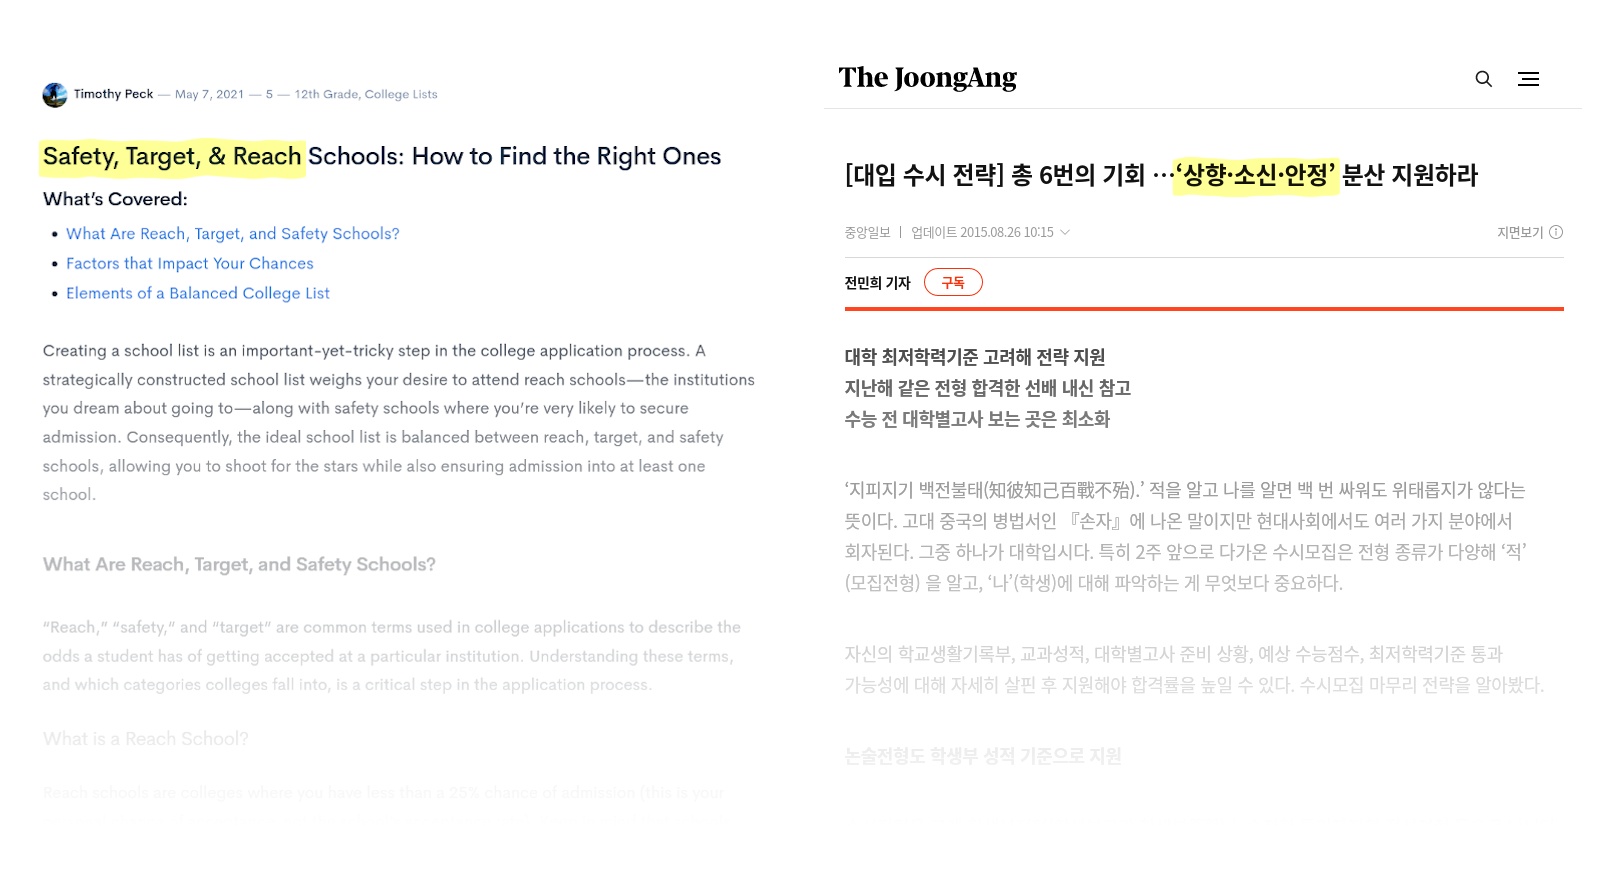
\includegraphics[width=\textwidth]{plots/news-both.png}

\ifen Do you trust the admissions consultant's advice?
\else 입학 컨설턴트의 조언, 믿을 만한가? \fi
\end{center}

\end{frame}







\begin{frame}[plain]{}
\begin{center}
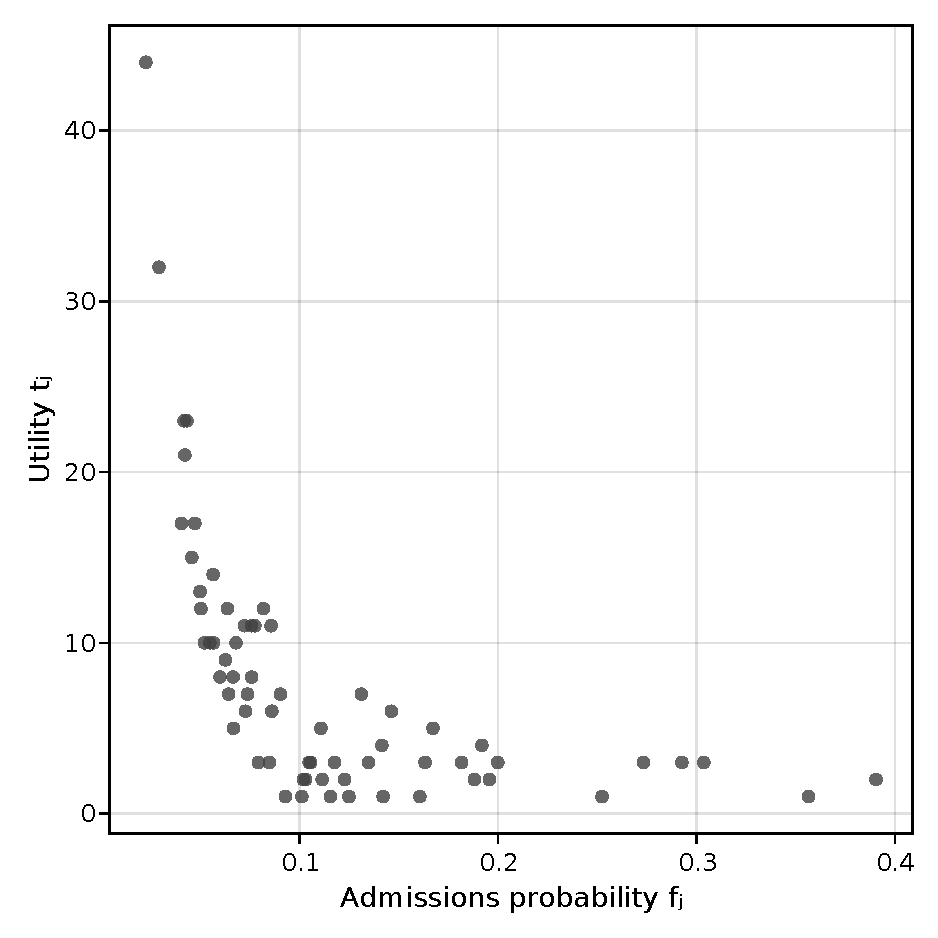
\includegraphics[height=\textheight]{plots/samplemarket.pdf}
\end{center}
\end{frame}





\begin{frame}[plain]{}
\begin{center}
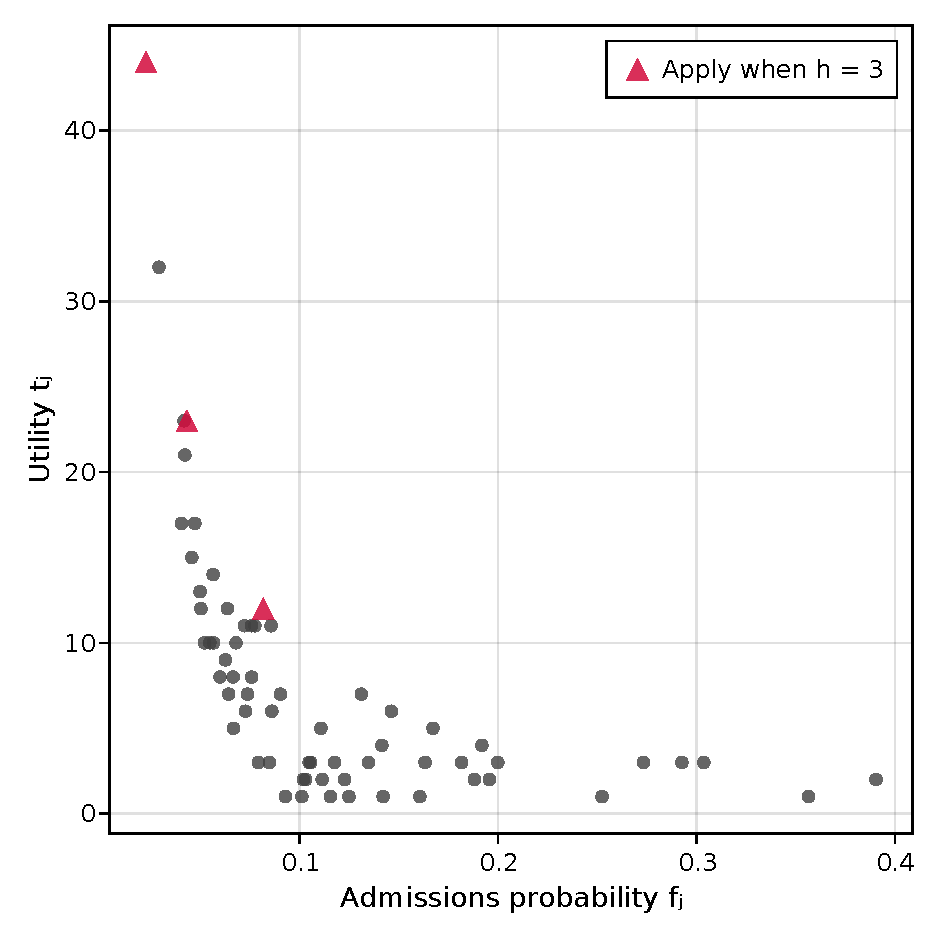
\includegraphics[height=\textheight]{plots/samplemarket-soln.pdf}
\end{center}
\end{frame}






\ifen {
\begin{frame}{Existing solutions}
In practice, most use \textbf{distributive heuristics} such as distributing applications evenly among reach, target, and safety schools. Turns out to be a \textbf{risk-averse} approach.

Another intuitive idea is the \textbf{linearization heuristic}. Since the expected utility associated with applying to $c_j$ (alone) is $f_j t_j$, solve the knapsack problem
\[\text{maximize}~~\sum_{j\in \mathcal{X}} f_j t_j \qquad \text{subject to}~~\sum_{j\in \mathcal{X}}g_j \leq H \]
as a surrogate. But this solution can be \textbf{arbitrarily bad}. 

Fu (2014) solved a similar problem by \textbf{enumeration}, which is intractable for $m \geq 20$ or so.

Our algorithms provide both \textbf{time and accuracy guarantees}. 
\end{frame}
} \else {
\begin{frame}{기존의 해법}
입학 컨설팅 산업에서는 주로 ``상향·소신·안정 지원 학교'' 각각 균일하게 지원하는 \textbf{배분적 휴리스틱}을 권장하며, 이는 \textbf{위험 회피적인} 전략임을 보일 수 있다. 

또한 $c_j$에만 지원할 때 기대 효용이 $f_j t_j$이므로 다음 배낭 문제를 대리 문제로 푸는 \textbf{선형화 휴리스틱}이 있다.
\[\text{maximize}~~\sum_{j\in \mathcal{X}} f_j t_j \qquad \text{subject to}~~\sum_{j\in \mathcal{X}}g_j \leq H \]
그러나 \textbf{최적해보다 아주 안 좋은 해를 출력할 수 있다}.

Fu (2014)는 비슷한 문제를 \textbf{열거법}으로 풀었으나, $m \geq 20$일 때 비현실적인 방법이다.

본 연구는 \textbf{계산 시간과 정확도가 보장된} 알고리즘을 제시한다. 
\end{frame}
} \fi













\ifen \section{Our algorithms} \else \section{알고리즘 제시} \fi

\ifen {
\begin{frame}[plain]
\begin{center}
~
\begin{beamercolorbox}[wd=.5\textwidth,sep=8pt,center,shadow=false,rounded=true]{section in head/foot}
    \usebeamerfont{title} \insertsectionhead
  \end{beamercolorbox}
\end{center}
\end{frame}
} \else {
\begin{frame}[plain]
\begin{center}
~
\begin{beamercolorbox}[wd=.5\textwidth,sep=8pt,center,shadow=false,rounded=true]{section in head/foot}
    \usebeamerfont{title} \insertsectionhead
  \end{beamercolorbox}
\end{center}
\end{frame}
} \fi





\ifen {
\begin{frame}{Overview of our algorithms}
We consider two cases of the college application problem:
\begin{itemize}
\item \textbf{Alma's problem:} Special case in which $g_j = 1$, i.e. a cardinality constraint instead of knapsack.

We provide an \textbf{exact, polynomial-time} solution via greedy algorithm.

\item \textbf{Ellis's problem:} The general case, which is NP-complete.

We provide four algorithms, including a \textbf{fully polynomial-time $(1 - \varepsilon)$-approximation algorithm}.
\end{itemize}

In general, submodular maximization over a knapsack constraint is $(1 - 1/e)$-inapproximable (Kulik et al. 2013), so the existence of an FPTAS for Ellis's problem is a significant result.
\end{frame}
} \else {
\begin{frame}{해법 개관}
대학 지원 문제를 2개의 경우로 나눌 수 있다.
\begin{itemize}
\item \textbf{알마의 문제:} 모든 $g_j = 1$, 즉 배낭 제약 대신 집합 크기 제약이 있는 특수한 경우.

\textbf{정확한 다항 시간} 탐욕 해법을 제시한다.

\item \textbf{엘리스의 문제:} NP-complete한 일반 경우.

총 4개의 해법을 제시하며, \textbf{완전 다항 시간 $(1 - \varepsilon)$-근사 해법}이 하이라이트다.
\end{itemize}

\looseness=-1
일반적으로, 배낭 제약식 위에서 submodular 함수를 최대화하는 문제는 $(1 - 1/e)$보다 좋은 근사 계수를 가지는 해법이 존재하지 않으므로 (Kulik et al. 2013), 엘리스 문제의 FPTAS가 존재하는 것은 의미가 있는 결과다.
\end{frame}
} \fi











\ifen
\section{Algos: Alma's problem}
\else
\section{해법 제시: 알마의 문제}
\fi

\ifen {
\begin{frame}{Alma's problem}
\dots is the \textbf{special case} in which each $g_j = 1$. 

Then $H$ is simply a limit on the number of schools you can apply to. This case mirrors the main Korean admissions cycle, in which $h = 3$ and $m= 202$. 

(In this case, we can assume that $H < m$; therefore, any polynomial in $H$ is bound by a polynomial in $m$. We  write $h$ in lowercase to emphasize this fact.)

Fisher et al. (1978) showed that a greedy algorithm is $(1 - 1/e)$-optimal for monotone submodular maximization. We show that the same algorithm is \emph{exact} for college application and improve its computation time. 
\end{frame}
} \else {
\begin{frame}{동일한 지원 비용의 경우}
``알마의 문제''란 \textbf{특수한 경우}에서 먼저 모든 $g_j = 1$이다.

이때 $H$는 단순한 지원 개수 제한이 되며, $h = 3, m = 202$인 한국 정시 입학 과정과 비슷한 상황이다.

(이 경우, $H < m$임을 가정할 수 있으므로 모든 $H$의 다항식에 대해 $m$의 다항식인 상한이 존재한다. 이를 강조하기 위해 $h$처럼 소문자로 표기한다.)

집합 크기 제약 위에 단조 submodular 함수를 최대화하는 문제에 대해, 탐욕 해법의 근가 계수가 $(1 - 1/e)$임이 알려져 있다 (Fisher 외 1978). 대학 지원 문제에 대해, 같은 해법이 정확한 해법임을 증명하고 계산 시간을 줄일 수 있다.
\end{frame}
} \fi







\ifen
\begin{frame}{Optimality of the greedy algorithm}
The following \textbf{nestedness property} for Alma's problem implies the optimality of a \textbf{greedy algorithm} that adds schools one at a time, maximizing $v(\mathcal{X})$ at each addition.
\begin{theorem}\label{nestedapplication}
There exists a sequence of portfolios $\{\mathcal{X}_h\}_{h=1}^m$ satisfying the nestedness relation
\begin{equation*}
\mathcal{X}_1 \subset \mathcal{X}_2\subset \dots \subset \mathcal{X}_m
\end{equation*}
such that each $\mathcal{X}_h$ is an optimal application portfolio when the application limit is $h$.
\end{theorem}

Using a variable-elimination technique, we reduce the cost of computing $v(\mathcal{X})$ to amortized unit time, obtaining an $O(hm)$ algorithm.
\end{frame}
\else
\begin{frame}{탐욕 해법의 정확성}
알마의 문제에 대해 다음 \textbf{포함 사슬 관계 (nestedness)} 성질은 $v(\mathcal{X})$를 최대화하는 순서대로 학교를 하나씩 추가하는 \textbf{탐욕 해법}의 최적성을 의미한다.
\begin{theorem}[최적 포트폴리오의 포함 사슬 관계] \label{nestedapplication}
각 $\mathcal{X}_h$가 지원 제한 $h$에 대한 최적 포트폴리오며 위의 포함 사슬 관계를 만족하는 포트폴리오 수열  $\{\mathcal{X}_h\}_{h=1}^m$가 존재한다.
\begin{equation*}
\mathcal{X}_1 \subset \mathcal{X}_2\subset \dots \subset \mathcal{X}_m
\end{equation*}
\end{theorem}

$v(\mathcal{X})$를 $O(1)$ 시간 안에 계산할 수 있는 변수 소거 기법을 개발하여 전체 해법의 계산 시간을 $O(hm)$으로 줄였다. 
\end{frame}
\fi






\ifen \section{Algos: Ellis's problem} \else \section{해법 제시: 엘리스의 문제} \fi

\ifen {
\begin{frame}{Algorithms for Ellis's problem}

By setting $f_j = \varepsilon$, we can make $v(\mathcal{X})$ arbitrarily close to a linear function. This means that knapsack reduces to Ellis's problem, and therefore Ellis's problem is NP-complete.

The general problem is \textbf{NP-complete} (reduction from knapsack). We offer four algorithms:
\begin{itemize}
\item A linear relaxation and \textbf{branch-and-bound scheme} allow us to interface with existing INLP solvers.

\item A \textbf{dynamic program based on total expenditures}. Exact solution in $O(Hm + m\log m)$ time (pseudopolynomial). 

\item A different DP based on truncated portfolio valuations. $(1 - \varepsilon)$-optimal solution in $O(m^3 / \varepsilon)$ time: an \textbf{FPTAS}!
\item A \textbf{simulated annealing heuristic}. Fast, typically within 2\% of optimality.
\end{itemize}
\end{frame}
} \else {
\begin{frame}{엘리스의 문제를 위한 알고리즘}

$f_j = \varepsilon$으로 넣으면 $v(\mathcal{X})$를 선형 함수에 원하는 만큼 가깝게 만들 수 있다. 배낭 문제가 엘리스의 문제로 변환할 수 있음을 의미하므로 엘리스의 문제는 NP-complete하다.

4개의 알고리즘 제시:
\begin{itemize}
\item 선형 완화 문제와 해당 \textbf{분지한계} (branch-and-bound) 해법. 일반적인 INLP 문제에 대해 자주 쓰이는 방법이다.

\item \textbf{총 지원 비용 기반 동적 계획}. $O(Hm + m\log m)$ (의사 다항) 시간에 정확한 해를 구하며, $g_j$가 작은 정수가 되는 ``전형적'' 인스턴스에 대해 매우 효율적인 해법.

\item 포트폴리오 가치의 라운딩을 이용한 동적 계획. $O(m^3 / \varepsilon)$ 시간에 $(1 - \varepsilon)$-근사해를 출력하므로 \textbf{FPTAS!}

\item \textbf{Simulated annealing} 휴리스틱. 빠르고 대부분 98\% 이상의 최적성을 얻었다.
\end{itemize}

\end{frame}
} \fi






\begin{frame}{\ifen Branch-and-bound algorithm: LP relaxation\else 분지한계법: 선형 완화 문제\fi}
\ifen
Our branch-and-bound framework is based on the following LP relaxation for Ellis's problem. 
\else
다음 선형 완화 문제 바탕으로 엘리스의 문제를 위한 분지한계법을 구성할 수 있다. 
\fi
\begin{problem}[\ifen LP relaxation for Ellis's problem\else 엘리스의 문제를 위한 선형 완화 문제\fi]\label{LPrelaxation}
\vspace{-2em}
\begin{align*}
\begin{split}
\text{maximize}\quad &  v_{\mathrm{LP}}(x) = \sum_{j=1}^m  f_j t_j x_j \\
\text{subject to}\quad & \sum_{j=1}^m g_j x_j \leq H, ~~ x \in [0, 1]^m
\end{split}
\end{align*}
\end{problem}
\ifen
We \textbf{tighten the LP bound} by recycling the variable-elimination technique from the proof of the nestedness theorem.

Problem \ref{LPrelaxation} is a continuous knapsack problem, easy to solve (Dantzig 1957; Balas and Zemel 1980). 
\else
포함 사슬 관계의 증명 과정에서 도출한 변수 소거법은 재활용해서 위에 \textbf{상한을 더 타이트하게} 조정한다.

문제 \ref{LPrelaxation}은 연속 배낭 문제로서 쉽게 풀 수 있다 (Dantzig 1957; Balas와 Zemel 1980). 
\fi
\end{frame}






\begin{frame}{\ifen Branch-and-bound algorithm: Possible improvements\else 분지한계법: 개선 방향\fi}
\ifen
A straightforward implementation is OK on small instances ($m \leq 35$), but leaves \textbf{considerable room for improvement} using better node-selection heuristics.

%The good news is that bespoke node-selection heuristics from the INLP literature typically require only a procedure for generating dual bounds from a constrained subproblem.

In the associated Julia package, we provide \textbf{modular containers for subproblems and their LP relaxations} that can interface with a more sophisticated branch-and-bound solver.

A branch-and-bound algorithm may be necessary to handle more advanced constraint structures.
\else
이 기반으로 만든 간단한 알고리즘은 작은 ($m \leq 35$) 인스턴스에 괜찮지만 분지 마디를 선택하는 휴리스틱으로 \textbf{개선할 여지가} 보인다.

Julia 코드 패키지에서 \textbf{부문제와 선형 완화 문제를 위한 modular한 데이터 구현을} 제시하며, 이를 더 세련된 INLP 솔버에 어렵지 않게 연결할 수 있다.

나중에 더 복합한 제약 조건을 도입하는 데에 분지한계법 알고리즘이 필요할 수 있으므로 유리하다.
\fi
\end{frame}








\begin{frame}{\ifen Expenditures-based dynamic program\else 지원 지출액 기반 동적 계획\fi}
\ifen Let $V[j,h] $ denote the value of the optimal portfolio that uses only the schools $\{ 1, \dots, j\}$ and costs no more than $h$.
\else $\{ 1, \dots, j\}$에 속한 학교만 사용하면서 지원 지출액이 $h$를 넘지 않은 최적 포트폴리오의 가치를 $V[j, h]$라고 하자.\fi

\ifen Then we can use the following \textbf{Bellman equation} to compute all the $V[j, h]$-values recursively.
\else 그러면 다음과 같은 \textbf{Bellman 식}으로 모든 $V[j, h]$-값은 재귀적으로 계산할 수 있다. \fi
\begin{align*}
V[j, h] = \max\bigl\{ V[j-1, h], (1 - f_j) V[j-1, h-g_j] + f_j t_j \bigr\}
\end{align*}
\ifen
This equation works because the $t_j$-values are indexed in ascending order.

Filling a lookup table with the $V[j, h]$-values therefore costs $O(Hm + m\log m)$, and then computing $\mathcal{X}$ is trivial.

\textbf{Very effective} on typical instances where $g_j$ are small integers.
\else
이 식의 타당성은 학교를 $t_j$-값 순서대로 배열함에 의존.

따라서 $V[j, h]$-값으로 표를 채우는 시간이 $O(Hm + m\log m)$이며 이를 참고하면 $\mathcal{X}$를 쉽게 구할 수 있다.

전형적인 인스턴스에서 $g_j$가 작은 상수이므로 \textbf{매우 효율적인} 해법.
\fi
\end{frame}








\begin{frame}{\ifen Valuation-based dynamic program: Fixed-point math \else 포트폴리오 가치 기반 동적 계획: 고정소숫점 산술 \fi}
\ifen 
As with the knapsack problem, Ellis's problem admits a \textbf{complementary dynamic program} that iterates on the value of the cheapest portfolio instead of on the cost of the most valuable portfolio.

We represent approximate portfolio valuations using a \textbf{fixed-point decimal} with a precision of $P$, where $P$ is the number of digits to retain after the decimal point. Let $r[x] =  10^{-P}\lfloor 10^P x \rfloor$ denote the value of $x$ rounded down to its nearest fixed-point representation.

$\bar U = \sum_{j\in \mathcal{C}} f_j t_j$ is an upper bound on the valuation of any portfolio, so the set $\mathcal{V}$ of possible valuations possible in the fixed-point framework is finite:
\else
엘리스의 문제는 배낭 문제와 같이, 가치가 가장 높은 포트폴리오의 비용 대신 비용이 가장 낮은 포트폴리오의 가치를 탐색하는 \textbf{보완적인 동적 계획}이 존재한다. 

포트폴리오의 근사적 가치를 정확도 $P$로 구성된 고정소수점 십진수(fixed-point decimal)로 나타내자. 다, $P$는 소수점 뒤에 등장하는 숫자의 수이다. 이때 $x$를 가장 가까운 고정소수점 십진수로 내림한 것을 $r[x] =  10^{-P}\lfloor 10^P x \rfloor$라고 하자.

임의의 포트폴리오의 가치가 $\bar U = \sum_{j\in \mathcal{C}} f_j t_j$를 넘을 수 없다. 따라서 고정소수점 환경에서 발생할 수 있는 포트폴리오 가치로 이루어진 집합 $\mathcal{V}$는 유한 집합이다.
\fi
\begin{equation*}
\mathcal{V} = \Bigl\{0, 1\times 10^{-P}, 2\times 10^{-P}, \dots, r\bigl[\bar U- 1\times 10^{-P}\bigr], r\bigl[\bar U\bigr]\Bigr\}
\end{equation*}
\ifen Then $|\mathcal{V} | = \bar U \times 10^P + 1$.
\else 그러면 $|\mathcal{V} | = \bar U \times 10^P + 1$이다.\fi

\end{frame}



\begin{frame}{\ifen Valuation-based dynamic program: Recursion relation \else 포트폴리오 가치 기반 동적 계획: 재귀 관계 \fi}
\ifen 
Let $G[j, v]$ denote the application cost of the least expensive portfolio that uses only schools $\{ 1, \dots, j\}$ and has (rounded) valuation at least $v$. We argue that
\else
$\{ 1, \dots, j\}$에 속한 학교만 사용하면 (내림한) 가치가 최소한 $v$의 포트폴리오 중 지원 비용이 최소한 포트폴리오의 지출액을 $G[j, v]$라고 하자. 이때 다음 재귀 관계가 성립한다고 주장한다.
\fi
\begin{align*}
G[j, v] &=
\begin{cases}
\infty, \quad & t_j < v \\
\min\bigl\{G[j-1, v], g_j + G[j-1, v - \Delta_j(v)] \bigr\}, \quad & t_j \geq v 
%\begin{cases}
%\min\bigl\{G[j-1, v], g_j + G[j-1, v - \Delta] \bigr\}, \quad &f_j < 1 \\
%\min\bigl\{G[j-1, v], g_j \bigr\}, \quad &f_j = 1 \text{ and } f_j t_j \geq v\\
%G[j-1, v], \quad &f_j = 1 \text{ and } f_j t_j < v
\end{cases}\\
\text{where}\quad
\Delta_j (v) &= 
\begin{cases}
r\left[\frac{f_j}{1 - f_j} (t_j - v)\right], \quad & f_j < 1\\
\infty, &f_j = 1\ifen.\fi
\end{cases} \label{deltajvdef}
\end{align*}

\ifen
Now we can fill a lookup table with the entries of $G[j, v]$ and compute an approximately optimal portfolio. 

In the paper, we show that setting $P \gets \bigl\lceil\log_{10}\left(m^2 / \varepsilon \bar U\right)\bigr\rceil$ guarantees a $(1- \epsilon)$-optimal portfolio, and that this yields a table of size $O(m^3 / \varepsilon)$, meaning that this algorithm is \textbf{an FPTAS}.
\else
이제 $G[j, v]$-값으로 표를 채우면 근사 최적 포트폴리오를 구할 수 있다.

논문에서 $P \gets \bigl\lceil\log_{10}\left(m^2 / \varepsilon \bar U\right)\bigr\rceil$로 넣으면 $(1- \epsilon)$-근사해가 보장되며, 해당 표의 크기가  $O(m^3 / \varepsilon)$이므로 이 알고리즘은 \textbf{FPTAS}이다.
\fi
\end{frame}





%Existence of FPTAS suggests college application is \textbf{a relatively easy instance of submodular maximization} (cf. Kulik et al. 2013).
%
%
%
%FPTAS의 존재성은 대학 지원 문제가 \textbf{submodular 최대화의 비교적 쉬운 인스턴스}임을 의미한다 (cf. Kulik 외 2013).






\begin{frame}{\ifen Simulated annealing algorithm \else Simulated annealing 해법 \fi}
\ifen {
SA is a familiar randomized technique for neighborhood search. 

No accuracy guarantee, but computation time is essentially negligible ⇒ popular in real-time applications such as vehicle routing where a ``good enough'' solution is needed quickly.

Ingredients for SA:
\begin{itemize}
\item An \textbf{initial solution}. We use the linearization heuristic, and solve the associated knapsack problem with the greedy heuristic.

\item A randomized procedure for \textbf{generating neighbors}. We add schools randomly until $\mathcal{X}$ becomes infeasible, then remove until feasibility restored.

\item \textbf{Temperature parameters} determine how likely the algorithm is to change candidates. $T =1/4$ and $r=1/16$ chosen by grid search.
\end{itemize}
} \else {
SA는 유명한 확률적 지역 탐색 기법이다.

정확도 보장은 없지만, 계산 시간이 아주 짧다. ⇒ 차량 라우팅처럼, ``충분히 좋은'' 해가 실시간에 필요한 분야에서 인기가 많다.

SA의 재료:
\begin{itemize}
\item \textbf{초기해}. 본 연구에서 선형화 휴리스틱을 적용하고 해당 배낭 문제를 탐욕 휴리스틱으로 풀어서 초기해를 구한다.

\item \textbf{해의 이웃해를 생성하는} 확률적 방법. $\mathcal{X}$의 가능성이 깨어질 때까지 학교를 무작위로 추가하고, 가능성이 복원될 때까지 무작위로 빼는 방법을 사용한다.

\item 해법이 이웃해로 바꾸는 확률을 결정하는 \textbf{온도 모수}. 그리드 탐색을 적용한 결과로 $T =1/4$ 그리고 $r=1/16$을 선택했다.
\end{itemize}
} \fi
\end{frame}






\ifen
\section{Computational results}
\else
\section{계산 실험 결과}
\fi

\ifen {
\begin{frame}[plain]
\begin{center}
~
\begin{beamercolorbox}[wd=.5\textwidth,sep=8pt,center,shadow=false,rounded=true]{section in head/foot}
    \usebeamerfont{title} \insertsectionhead
  \end{beamercolorbox}
\end{center}
\end{frame}
} \else {
\begin{frame}[plain]
\begin{center}
~
\begin{beamercolorbox}[wd=.5\textwidth,sep=8pt,center,shadow=false,rounded=true]{section in head/foot}
    \usebeamerfont{title} \insertsectionhead
  \end{beamercolorbox}
\end{center}
\end{frame}
} \fi





\ifen {
\begin{frame}{Experimental procedure}
\textbf{Three computational experiments} designed to test the efficiency and accuracy of our solution algorithms.

Recipe for an experimental instance with $m$ schools:
\begin{itemize}
\item Each $t_j$ drawn from an exponential distribution.
\item $f_j$ chosen to correlate with $1/ t_j$ (creates reach/safety schools).
\item Alma's problem: $h = \lfloor m/2 \rfloor$.
\item Ellis's problem: $g_j$ small integers, $H = \lfloor \frac{1}{2} \sum g_j\rfloor$.
\end{itemize}

\looseness=-1
All algorithms implemented and tested in Julia (v1.8.0b1). Code available on Github (Kapur 2022) and in Julia registry (OptimalApplication.jl). 


\end{frame}
} \else {
\begin{frame}{실험 방법}
해법의 효율성과 정확성을 탐구하고자 \textbf{3개의 계산 실험을} 진행했다.

$m$개의 학교로 구성된 가상 인스선트 레시피:
\begin{itemize}
\item 각 $t_j$는 지수 분포에서 생성한다.
\item (상향/안정 지원 학교를 만들기 위해) $1 / t_j$과 비례하도록 $f_j$를 생성한다.
\item 알마의 문제: $h = \lfloor m/2 \rfloor$.
\item 엘리스의 문제: $g_j$ 작은 정수, $H = \lfloor \frac{1}{2} \sum g_j\rfloor$.
\end{itemize}

모든 알고리즘은 Julia (v1.8.0b1) 언어로 구현했다. Github 리포 (Kapur 2022) 혹은 Julia 패키지 등록 (OptimalApplication.jl)에서 코드를 공유한다.
\end{frame}
} \fi











\begin{frame}{\ifen Experiment 1 \else 실험 1 \fi}
\ifen 
\dots compares \textbf{two data structures} for the greedy algorithm for Alma's problem. 
 
50 markets in each cell, time recorded as best of three reps. Table shows mean (std) computation time in ms.
\else
실험 1에서 알마 문제의 탐욕 해법을 위한 \textbf{2개의 데이터 구현을} 비교한다.

\looseness=-1
각 칸에서 50개의 시장을 생성하고 최적해를 3번 계산한 것 중에 최소 시간을 기록. 표에서 나타나는 값은 평균 (표준편차) 시간이며 단위는 ms.
\fi
\begin{center}
\scalebox{0.92}{ %
\begin{tabular}{r|r@{~}r|r@{~}r}
\ifen 
 \textbf{\begin{tabular}[r]{@{}r@{}}\\$m$\end{tabular}}& \multicolumn{2}{c|}{\textbf{\begin{tabular}[c]{@{}c@{}}Greedy alg.\\with list\end{tabular}}}  & \multicolumn{2}{c}{\textbf{\begin{tabular}[c]{@{}c@{}}Greedy alg.\\with heap\end{tabular}}}\\ \hline
 \else
 \textbf{\begin{tabular}[r]{@{}r@{}}\\$m$\end{tabular}}& \multicolumn{2}{c|}{\textbf{\begin{tabular}[c]{@{}c@{}}탐욕 알고리즘\\(목록 구현)\end{tabular}}}  & \multicolumn{2}{c}{\textbf{\begin{tabular}[c]{@{}c@{}}탐욕 알고리즘\\(힙 구현)\end{tabular}}}\\ \hline
 \fi
    16 &           0.00 &        (0.00) &           0.01 &        (0.00) \\
    64 &           0.03 &        (0.00) &           0.08 &        (0.02) \\
   256 &           0.15 &        (0.01) &           0.97 &        (0.22) \\
  1024 &           2.31 &        (0.05) &          14.44 &        (1.66) \\
  4096 &          37.85 &        (0.61) &         245.74 &       (17.33) \\
 16384 &         585.75 &        (2.11) &        4728.59 &      (552.25)
\end{tabular}
}
\end{center}
\ifen 
$\argmax$ operation at each iteration made heap an appealing data structure, but because \emph{every} key is updated, the savings aren't worth the cost.
\else 
반복 단계마다 $\argmax$ 연산이 필요하므로 힙 구현에는 매력이 있지만, 그의 모든 원소를 수정해야 하므로 만회하지 않는다.
\fi

\end{frame}




\begin{frame}{\ifen Experiment 2\else Experiment 2\fi}
\ifen 
\dots compares the speed of \textbf{guaranteed-accuracy} algorithms for Ellis's problem.
\else 
실험 2에서 엘리스 문제를 위한 \textbf{정확도가 보장된} 해법의 계산 시간을 비교한다.
\fi
\begin{center}
\resizebox{\textwidth}{!}{ %
\begin{tabular}{r|r@{~}r|r@{~}r|r@{~}r|r@{~}r} %
\ifen %
\textbf{\begin{tabular}[r]{@{}r@{}}$m$\end{tabular}}&\multicolumn{2}{c|}{\textbf{\begin{tabular}[c]{@{}c@{}}Branch \& bound\end{tabular}}}  & \multicolumn{2}{c|}{\textbf{\begin{tabular}[c]{@{}c@{}}App. costs DP\end{tabular}}}  &\multicolumn{2}{c|}{\textbf{\begin{tabular}[c]{@{}c@{}}FPTAS, $\varepsilon= 0.5$\end{tabular}}}  & \multicolumn{2}{c}{\textbf{\begin{tabular}[c]{@{}c@{}}FPTAS, $\varepsilon= 0.05$\end{tabular}}}   \\ \hline
\else
\textbf{\begin{tabular}[r]{@{}r@{}}$m$\end{tabular}}&\multicolumn{2}{c|}{\textbf{\begin{tabular}[c]{@{}c@{}}분지한계법\end{tabular}}}  & \multicolumn{2}{c|}{\textbf{\begin{tabular}[c]{@{}c@{}}지출액 DP\end{tabular}}}  &\multicolumn{2}{c|}{\textbf{\begin{tabular}[c]{@{}c@{}}FPTAS, $\varepsilon= 0.5$\end{tabular}}}  & \multicolumn{2}{c}{\textbf{\begin{tabular}[c]{@{}c@{}}FPTAS, $\varepsilon= 0.05$\end{tabular}}}   \\ \hline
\fi
     8 &          0.04 &       (0.02) &         0.01 &      (0.00) &                0.05 &             (0.01) &                 0.21 &              (0.06) \\
    16 &          0.22 &       (0.11) &         0.07 &      (0.01) &                0.43 &             (0.10) &                 3.15 &              (0.74) \\
    32 &        166.20 &     (422.31) &         0.31 &      (0.05) &                2.38 &             (0.38) &                33.38 &             (11.68) \\
    64 &             — &          (—) &         1.36 &      (0.18) &               15.32 &             (2.77) &               405.73 &            (125.98) \\
   128 &             — &          (—) &         6.52 &      (0.72) &               84.50 &            (22.59) &              2362.19 &           (1095.11) \\
   256 &             — &          (—) &        31.23 &      (1.91) &             1085.60 &          (1186.24) &             22129.92 &           (6588.40)
\end{tabular}
}
\end{center}
\ifen 
\textbf{Costs DP has a pronounced advantage} because $g_j$ are small integers.

Bottleneck for FPTAS is computer memory rather than time. 
\else
실험 데이터에서 $g_j$가 작은 정수이므로 \textbf{지원 지출액 기반 동적 계획은 상당한 우위}를 발휘한다. 

FPTAS의 병목 요소는 계산 시간이 아니라 메모리 소모량.
\fi

\end{frame}





\begin{frame}{Experiment 3}
\ifen
\dots investigates the \textbf{empirical accuracy} of the simulated annealing heuristic in 500 synthetic instances.
\else
실험 3에서 simulated annealing 해법의 \textbf{실무적 정확도를} 가상 인스턴스를 통해 탐구한다.
\fi
\begin{center}
 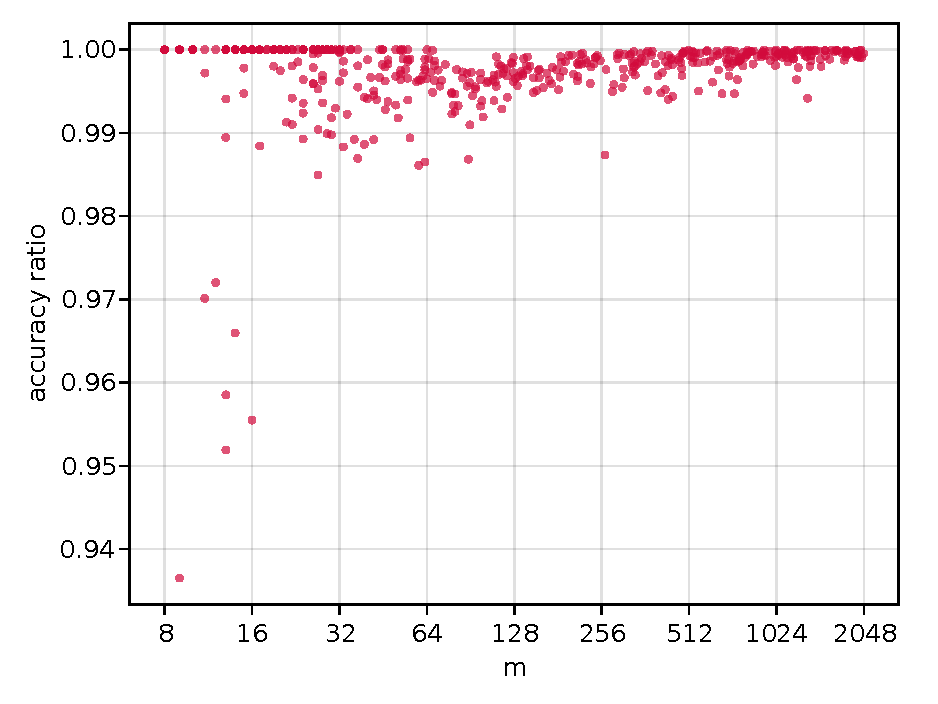
\includegraphics[height=18em]{./plots/accuracy_simulatedannealing.pdf}
\end{center}
\end{frame}









\ifen \section{Conclusion} \else \section{결론} \fi

\ifen {
\begin{frame}[plain]
\begin{center}
~
\begin{beamercolorbox}[wd=.5\textwidth,sep=8pt,center,shadow=false,rounded=true]{section in head/foot}
    \usebeamerfont{title} \insertsectionhead
  \end{beamercolorbox}
\end{center}
\end{frame}
} \else {
\begin{frame}[plain]
\begin{center}
~
\begin{beamercolorbox}[wd=.5\textwidth,sep=8pt,center,shadow=false,rounded=true]{section in head/foot}
    \usebeamerfont{title} \insertsectionhead
  \end{beamercolorbox}
\end{center}
\end{frame}
} \fi






\ifen {
\begin{frame}{Conclusion}
``Maximax'' form, integrality constraints make the college application problem \textbf{theoretically interesting}. Formally, it is a submodular maximization problem, but its approximability is more like knapsack (cf.~Fisher et al. 1978; Kulik et al. 2013; Kellerer et al. 2004).

% I decided I don't like this sentence bc the claim is obvious and the claim that the proof is ``subtle'' is subjective.
%The nestedness result for the $g_j = 1$ special case also resembles the knapsack problem, although the proof is more subtle. 

\looseness=-1
Solutions to the college application problem have \textbf{practical value}: US admissions consultants charge an average of \$200/hr (Sklarow 2018)!

⇒ Open-sourcing our code for public benefit (Kapur 2022).

\textbf{Possible extensions} of our model:
\begin{itemize}
\item Explicit treatment of risk aversion as in the classic Markowitz (1952) model.
\item Diversification constraints like Korea's application fields.
\item Reduce memory usage of dynamic programs. 
\end{itemize}
\end{frame}
} \else {
\begin{frame}{결론}
\looseness=-1
``Maximax'' 형태와 정수 조건 때문에 대학 지원 문제는 \textbf{이론적으로 흥미로운 문제이다}. Submodular 최대화 문제지만, 근사 해법의 성질은 배낭 문제에 더 가깝다 (cf. Fisher 외 1978; Kulik 외 2013; Kellerer 외 2004).

%$g_j=1$의 특수한 경우의 포함 사슬 관계 성질도 배낭 문제와 유사하며, 증명 과정은 좀 더 미묘하다.

좋은 대학 지원 전략에는 \textbf{금전적 가치가 있다}. 미국 입학 컨설턴트의 시간당 급료는 평균 200달러 (Sklarow 2018)!

\mbox{⇒ 공공 이익을 위해 코드는 open-source license로 공개 (Kapur 2022).}

\textbf{향후 연구:}
\begin{itemize}
\item 고전적 Markowitz (1952)자산배분 모형처럼, 위험 회피를 명시적으로 다루는 새로운 목적함수.
\item 한국 입학 과정의 가나다군과 같은 다각화 제약 조건.
\item 동적 계획의 메모리 소모량 절감. 
\end{itemize}
\end{frame}
} \fi







\begin{frame}[allowframebreaks]{\ifen References \else 참고 문헌 \fi}
\parskip 0em
\leftskip 2em
\parindent -2em
Balas, Egon and Eitan Zemel. 1980. ``An Algorithm for Large Zero-One Knapsack Problems.'' \emph{Operations Research} 28 (5): 1130--54. \url{https://doi.org/10.1287/opre.28.5.1130}. 

Dantzig, George B. 1957. ``Discrete-Variable Extremum Problems.'' \emph{Operations Research} 5 (2): 266--88.

Fisher, Marshall, George Nemhauser, and Laurence Wolsey. 1978. ``An analysis of approximations for maximizing submodular set functions—I.'' \emph{Mathematical Programming} 14: 265--94. 

Fu, Chao. 2014. ``Equilibrium Tuition, Applications, Admissions, and Enrollment in the College Market.'' \emph{Journal of Political Economy} 122 (2): 225--81. \url{https://doi.org/10.1086/675503}. 

Kapur, Max. 2022. ``OptimalApplication.'' GitHub repository. \url{https://github.com/maxkapur/OptimalApplication.jl}.

%Kapur, Max and Sung-Pil Hong. 2022. ``The College Application Problem.'' Preprint. \url{https://arxiv.org/abs/2205.01869}.

\framebreak

Kellerer, Hans, Ulrich Pferschy, and David Pisinger. 2004. \emph{Knapsack Problems.} Berlin: Springer.

Kulik, Ariel, Hadas Shachnai, and Tami Tamir. 2013. ``Approximations for Monotone and Nonmonotone Submodular Maximization with Knapsack Constraints.'' \emph{Mathematics of Operations Research} 38 (4): 729--39. \url{https://doi.org/10.1287/moor.2013.0592}.

Markowitz, Harry. 1952. ``Portfolio Selection.'' \emph{The Journal of Finance} 7 (1): 77--91. \url{https://www.jstor.org/stable/2975974}.

%Rozanov, Mark and Arie Tamir. 2020. ``The nestedness property of the convex ordered median location problem on a tree.'' \emph{Discrete Optimization} 36: 100581. \url{https://doi.org/10.1016/j.disopt.2020.100581}.

Sklarow, Mark. 2018. \emph{State of the Profession 2018: The 10 Trends Reshaping Independent Educational Consulting.} Technical report, Independent Educational Consultants Association. \url{https://www.iecaonline.com/wp-content/uploads/2020/02/IECA-Current-Trends-2018.pdf}.

\end{frame}








\ifen \section{Appendix} \else \section{부록} \fi

\begin{frame}{\ifen Summary of algorithms\else 알고리즘 요약\fi}
\begin{center}
\ifen
\scalebox{0.90}{ 
\begin{tabular}{r|lllll}
\textbf{Algorithm} & \textbf{Problem} & \textbf{Restrictions} & \textbf{Exactness}       & \textbf{Computation time} \\ \hline
\xrowht[()]{1.5em}  \begin{tabular}[r]{@{}r@{}}Na\"ive\end{tabular} &  \begin{tabular}[l]{@{}l@{}}Homogeneous \\ costs\end{tabular}     & None                  & $(1/h)$-opt.               & $O(m)$                    \\ 
\xrowht[()]{1.5em}  Greedy                &   \begin{tabular}[l]{@{}l@{}}Homogeneous \\ costs\end{tabular}    & None                  & Exact                    & $O(hm)$                   \\
\xrowht[()]{1.5em}  \begin{tabular}[r]{@{}r@{}}Branch and\\ bound\end{tabular}   & General          & None                  & Exact                    & $O(2^m)$                  \\
\xrowht[()]{1.5em}  Costs DP     &   General          & $g_j$ integer         & Exact                    & $O(Hm + m \log m)$        \\
\xrowht[()]{1.5em}  FPTAS      &   General          & None        & $(1 - \varepsilon)$-opt. & $O(m^3 / \varepsilon)$   \\
\xrowht[()]{1.5em}  \begin{tabular}[r]{@{}r@{}}Simulated\\annealing\end{tabular}   & General          & None                  & $0$-opt.                    & $O(Nm)$                
\end{tabular}
}
\else
\scalebox{1}{ 
\begin{tabular}{r|lllll}
\textbf{알고리즘} &  \textbf{문제} & \textbf{제한} & \textbf{정확도}       & \textbf{계산 시간} \\ \hline
\xrowht[()]{1.7em}  \begin{tabular}[r]{@{}r@{}}나이브\end{tabular}                & \begin{tabular}[l]{@{}l@{}}동일한\\ 지원 비용\end{tabular}     & 없음                  & $(1/h)$-근사          & $O(m)$                    \\ 
\xrowht[()]{1.7em}  탐욕 해법               &  \begin{tabular}[l]{@{}l@{}}동일한\\ 지원 비용\end{tabular}    & 없음                  & 정확                    & $O(hm)$                   \\
\xrowht[()]{1.7em}  \begin{tabular}[r]{@{}r@{}}Branch and\\ bound\end{tabular}   & 일반 문제          & 없음                  & 정확                    & $O(2^m)$                  \\
\xrowht[()]{1.7em}   \begin{tabular}[r]{@{}r@{}}지원 비용\\ 동적 계획\end{tabular}    & 일반 문제          & $g_j$ 정수         & 정확                    & $O(Hm + m \log m)$        \\
\xrowht[()]{1.7em}  FPTAS       & 일반 문제          & 없음        & $(1 - \varepsilon)$-근사 & $O(m^3 / \varepsilon)$   \\
\xrowht[()]{1.7em}   \begin{tabular}[r]{@{}r@{}}Simulated\\ annealing\end{tabular}    & 일반 문제          & 없음                      & $0$-근사                    & $O(Nm)$                
\end{tabular}
}
\fi
\end{center}
\end{frame}








\ifen {
\begin{frame}{A small example}
College data and optimal application portfolios for a fictional market with $m=8$ schools.
\vspace{-1em}
\begin{center}
\begin{tabular}{r|lcccc}
\textbf{$j$} & \textbf{School $c_j$} & \textbf{Admit prob. $f_j$} & \textbf{Utility $t_j$} & \textbf{Priority} & \textbf{$v(\mathcal{X}_h)$} \\ \hline
\\[-.75em]
1 & Mercury University  & 0.39   & 200 & 4   & 230.0   \\
2 & Venus University    & 0.33   & 250 & 2   & 146.7  \\
3 & Mars University     & 0.24   & 300 & 6   & 281.5  \\
4 & Jupiter University  & 0.24   & 350 & 1   & \phantom{0}84.0  \\
5 & Saturn University   & 0.05   & 400 & 7   & 288.8  \\
6 & Uranus University   & 0.03   & 450 & 8   & 294.1  \\
7 & Neptune University  & 0.10   & 500 & 5   & 257.7  \\
8 & Pluto College       & 0.12   & 550 & 3   & 195.1      
\end{tabular}
\end{center}
By the nestedness property, the optimal portfolio when the application limit is $h$ consists of the $h$ schools having priority $h$ or less.

Valuation function appears on next slide. Always concave.
\end{frame}
} \else {
\begin{frame}{작은 예제}
$m=8$개의 학교로 이루어진 가상 입학 시장의 대학교 자료와 최적 지원 포트폴리오.
\begin{center}
\begin{tabular}{r|lcccc}
\textbf{지표 $j$} & \textbf{학교 $c_j$} & \textbf{합격 확률 $f_j$} & \textbf{효용 $t_j$}  & \textbf{지원 순위} & \textbf{$v(\mathcal{X}_h)$} \\ \hline
\\[-.75em]
1 & 수성대   & 0.39   & 200 & 4   & 230.0   \\
2 & 금성대   & 0.33   & 250 & 2   & 146.7  \\
3 & 화성대   & 0.24   & 300 & 6   & 281.5  \\
4 & 목성대   & 0.24   & 350 & 1   & \phantom{0}84.0  \\
5 & 토성대   & 0.05   & 400 & 7   & 288.8  \\
6 & 천왕성대  & 0.03   & 450 & 8   & 294.1  \\
7 & 해왕성대  & 0.10   & 500 & 5   & 257.7  \\
8 & 명왕성대  & 0.12   & 550 & 3   & 195.1      
\end{tabular}
\end{center}
포함 사슬 관계 성질에 따라, 지원 제한이 $h$일 때 최적 포트폴리오는 지원 순위가 $h$ 이하인 $h$개의 학교로 구성된다.
\end{frame}
} \fi












\begin{frame}[plain]
\begin{center}
 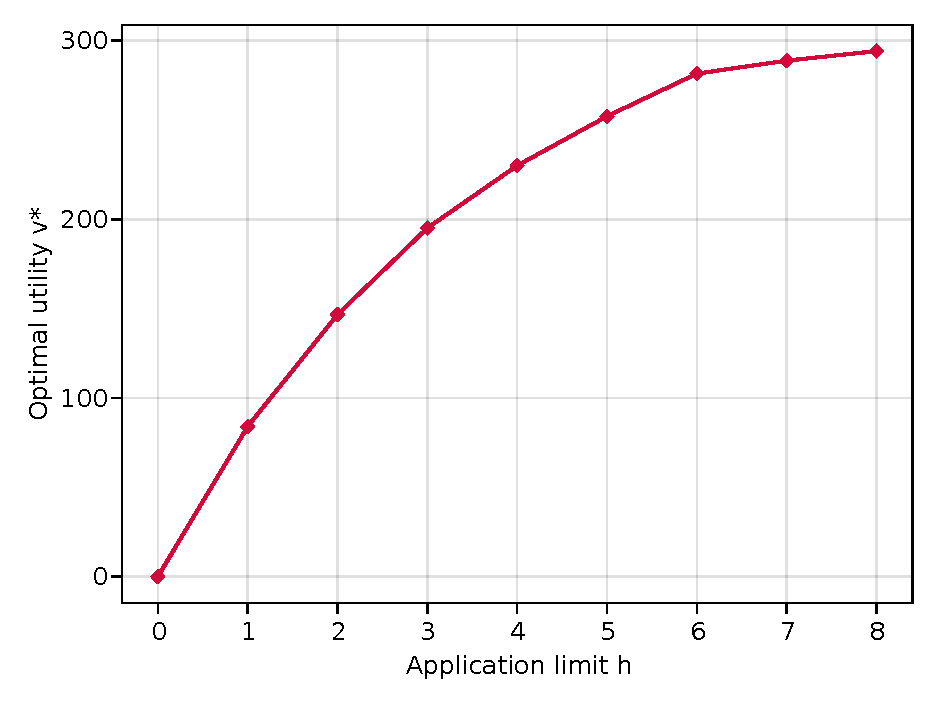
\includegraphics[height=\textheight]{./plots/h_v-example.pdf}
\end{center}
\end{frame}








\end{document}
